 \section{Mappings} \label{sec:mappings}
Fran\c{c}ois Faure

% % mappings
\newcommand{\JNL}{\ensuremath{\mathcal{J}}}     % positions
\newcommand{\J}{\ensuremath{J}}     % mapping lineaire

\newcommand{\mass}{\ensuremath{M}}             % matrice de masse
\newcommand{\vol}{\ensuremath{\mathcal V}} % volume d'intersection
\newcommand{\press}{\ensuremath{\rho}}

% In section~\ref{sec:pixelcontact}, we have shown how to efficiently compute repulsion forces between arbitrary polyhedra.
% In this section, we present a general framework to map the contact forces to the degrees of freedom of arbitrary physical models.
% We then demonstrate it on a variety of models.

\subsection{Motivation} \label{sec:geometryLayers}
Different geometrical models can be used to model objects in contact.
We organize them in a hierarchy of layers. An example is shown in figure~\ref{fig:hierarchy}, where a rigid object hits a shape embedded in deformable cells.

\begin{figure}
 \centering
 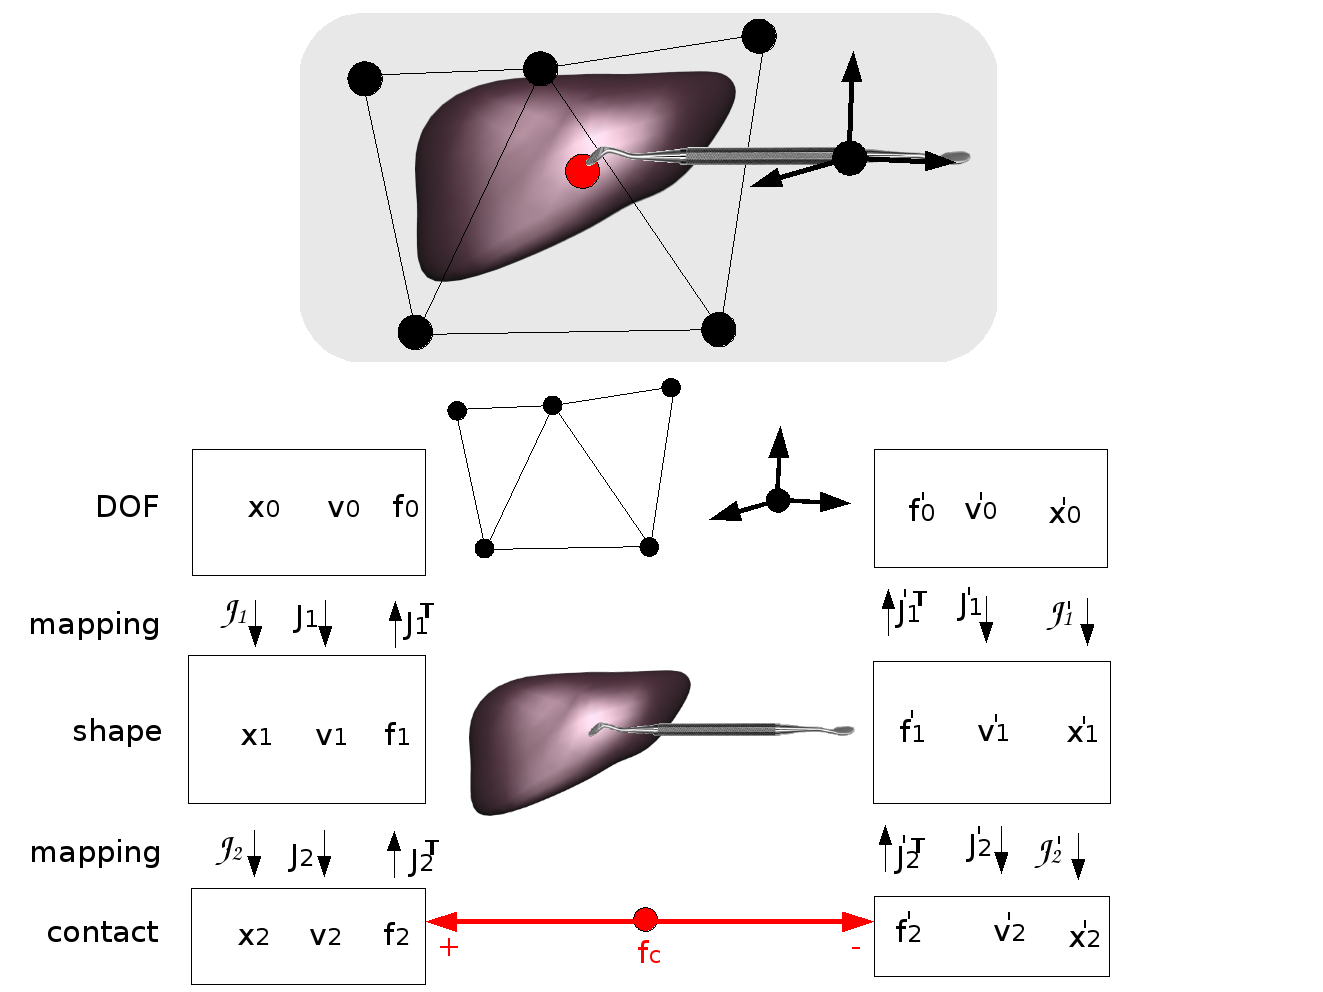
\includegraphics[width=\linewidth]{mappings.png}
 \caption{Mappings from the DOFs to a contact point. Top: two simulated objects in contact (red point). Bottom: hierarchy of geometrical layers. Positions and velocities are propagated top-down. The contact force $f_c$ is accumulated in the contact layers. Forces are then propagated bottom-up.
%Each object has its own state vectors and mappings.
}
 \label{fig:hierarchy}
\end{figure}

% bases de la dynamique
The state of a simulated system can be described by the values and time derivatives of its independent degrees of freedom (DOF) gathered in two vectors $x_0$ and $v_0$.
The dynamics equation (Newton's law) relates the second time derivative $a_0$ of the DOF to the forces $f_0$ acting on them: $f_0 = \mass a_0$, where \mass~ is a matrix modeling the mass of the system.
%We call $f_0$ the \textit{net force}.

% attacher de la g�om�trie
Geometry can be attached to the DOF for visualization or contact computation. 
We call it the \textit{shape}.
It is typically defined by points, such as triangle vertices or sphere centers, and additional data such as triangle connectivity or sphere radii.
We call these points the \textit{vertices}. 
Their positions, velocities and associated forces are stored in vectors $x_1$, $v_1$ and $f_1$, respectively.
They are not independent variables, since the positions and velocities are bound to the DOF.
We say that the geometrical model $1$ is mapped from model $0$,
 using a kinematic operator which we call \textit{mapping}:
\begin{eqnarray*} %\label{eq:mapV}
x_1 &=&\JNL_1(x_0)\\ 
v_1 &=& J_1 v_0
\end{eqnarray*}
Typical mappings include polygonal shapes attached to rigid bodies using local coordinates, or embedded in deformable cells using barycentric coordinates, as well as skin surrounding articulated bodies using vertex blending techniques.
Matrix $J_1 = \frac{\partial x_1}{\partial x_0}$ encodes the linear relation between the DOF velocities and the shape velocities. Due to linearity, the same relation holds on elementary displacements $dx$.
It also holds on accelerations, with an additional offset due to velocities when the position mapping \JNL is nonlinear.
In most cases, operators \JNL~ and \J~ are the same, but in the case of rigid bodies, \JNL~ is nonlinear with respect to $x$ and it can not be written as a matrix.
For surfaces embedded in deformable cells, matrix \J~contains the barycentric coordinates. 
For surfaces attached to rigid bodies, each row of the matrix encodes the usual relation $v = \dot o + \omega \times (x-o)$ for each vertex. 
Similarly, skins around articulated bodies involve, at each vertex, the weighted  contributions of the rigid bodies. 


% g�om�trie suppl�mentaire d�e aux contacts
When shapes collide, additional geometry can be necessary to model the contact.
For instance, when an edge intersects another one, a contact force is applied to the intersection points.
These points are defined by their barycentric coordinates with respect to their edge vertices. Other relations can be used, depending on the kind of geometrical primitives in contact.
This additional geometry requires another geometrical layer connected to the shape by a mapping, as illustrated in figure~\ref{fig:hierarchy}.
% This layer is also connected to the shape using mappings:
% \begin{eqnarray*} %\label{eq:mapV}
% x_2 &=&\JNL_2(x_1)\\ 
% v_2 &=&J_2 v_1 
% \end{eqnarray*}

We can straightforwardly extend this approach to tree-like hierarchies of geometries, with the DOF layer at the root. 
For instance, the DOF layer may have two independent children, one for collision using a coarse mesh, and the other for rendering using a finer mesh. The synchronization between these sibling layers is automatically guaranteed by their attachment to their common ancestor, the DOF layer.
The hierarchy can also be deeper, using for instance a fine mesh for rendering and its convex hull for collision.
This flexible framework gives us a great freedom for physical modeling.

\subsection{Mappings}
Positions and velocities can be propagated top-down through a hierarchy of geometrical models using the relations presented in the previous section. Conversely,
in order to take the contact forces into account in the dynamics equation, we need to propagate the forces bottom-up in the hierarchy, up to the independent DOFs, on which Newton's law $f=ma$ is applied. 
Moreover, implicit differential equation solvers need compute changes of force  given changes of displacements, and constraint solvers need to translate the expression of constraint Jacobian from lower models to the top.
% The mapping methods are organized in three categories:
% - method apply propagates positions top-down and computes derivatives of the mapping functions
% - methods applyJ() 

Given forces $f_n$ applied to a geometrical model $n$, the mapping computes and accumulates the equivalent force applied to its parent model $n-1$. 
Since equivalent forces must have the same power, we have to compute $f_{n-1}$ such that:
$$
v_{n-1}^T f_{n-1} = v_n^T f_n
$$
The kinematic relation $v_{n} = J_{n}v_{n-1}$ allows us to rewrite the previous equation as
$$
v_{n-1}^T f_{n-1} = v_{n-1}^T J_{n}^T f_n
$$
Since this relation must hold for any velocity $v_{n-1}$, the principle of virtual work allows us to simplify the previous equation to obtain:
\begin{equation} \label{eq:mapF}
f_{n-1} = J_n^T f_n
\end{equation}
The name of the methods used to propagate velocities or small displacements top-down contain $J$, which denotes the kinematic matrix, while the names of the methods used to propagate forces or constraint Jacobians bottom-up contain $JT$, which denotes the transpose of the same.
Method \texttt{applyJT( OutDataVecDeriv\& out, const InDataVecDeriv\& in, const MechanicalParams* mparams)} is used to accumulate forces from a child model to its parent. It performs a cumulative write (+=) since a model may have several children:
\begin{equation}
 \label{eq.applyjt}
 f_{n-1} += J_n^T f_n
\end{equation}

Some differential equation solvers need compute the change of force df, given a change of position dx.
The displacement dx, considered small, is propagated top-down using the linear operator \texttt{applyJ( InDataVecDeriv\& out, const OutDataVecDeriv\& in, const MechanicalParams* mparams)}, then the force changes are accumulated bottom-up.
Differentiating eq.\ref{eq.applyjt}, we get:
\begin{equation}
 \label{eq.applydjt}
 \delta f_{n-1} += J_n^T \delta f_n + \delta J_n^T f_n
\end{equation}
Once the change of child force $delta f_n$ is computed (see the section on force fields), method \texttt{applyJT} is used to accumulate it in the parent, corresponding to the first term in the right of eq.\ref{eq.applydjt}.
Method \texttt{applyDJT(MultiVecDerivId parentForce, ConstMultiVecDerivId  childForce, const MechanicalParams* mparams  )} is used to accumulate the second term, which is due to the change of matrix J due to a displacement.
It is null in linear mappings, such as BarycentricMapping.
The method queries the last displacement propagated using the MechanicalParams.

Nonlinearity is also implied in the computation of accelerations.
The top-down method to compute the nonlinear, velocity-dependent part of accelerations is \texttt{computeAccFromMapping(MultiVecDerivId outAcc, ConstMultiVecDerivId inVel, ConstMultiVecDerivId inAcc, const MechanicalParams* mparams )}.

Constraints enforced using Lagrange multipliers are represented using linear equations.
When these are applied to child models, method \texttt{applyJT( InDataMatrixDeriv\& out, const OutDataMatrixDeriv\& in, const ConstraintParams* mparams )} is used to propagate the Jacobians bottom-up.



%This simple relation allows us to map forces bottom-up through the hierarchy. 
%The corresponding acceleration can then be computed in the DOF layer.

% We emphasize the simplicity and the generality of equation~\ref{eq:mapF}. 
% It makes no assumption about the constitutive laws of the simulated objects.
% It allows us to connect arbitrary bodies using any geometry, provided that a kinematic operator linking the velocity of the geometry to the body DOFs is available.
% %It is not limited to polygonal geometries.

% It encompasses and generalizes \cite{Sifakis07}'s hard bindings which were introduced for Finite Elements and empirically extended to rigid bodies.
% It enables us to efficiently and straightforwardly connect or make collide a wide variety of bodies.

% Let $x_n$, $y_n$, $f_n$ be, respectively, the positions, velocities and net forces in the geometrical model $n$, and $x_{n+1}$, $y_{n+1}$, $f_{n+1}$ the positions, velocities and net forces in model $n+1$ mapped from model $n$.
% The mappings have the following propagation methods:
% \begin{itemize}
%  \item apply: propa
% \end{itemize}


